\def\pgfsysdriver{pgfsys-dvisvgm.def}
% flashcards-title: Cross-scale plant-system synthesis
% flashcards-desc: Dry soil and hot air point to reduced water input and increased water loss in one plant, leading to drooping. A population panel shows varied responses, with a dashed arrow to population change labeled more evidence needed.
\documentclass[tikz,border=6pt]{standalone}
\usetikzlibrary{arrows.meta,calc,fit,positioning,shapes.geometric}

\definecolor{fcink}{HTML}{17212B}
\definecolor{fcblue}{HTML}{1D5D8C}
\definecolor{fcgreen}{HTML}{2D6A4F}
\definecolor{fcorange}{HTML}{A44A1F}
\definecolor{fcpale}{HTML}{F4F7F9}
\definecolor{fcsoil}{HTML}{8B5E3C}

\tikzset{
  fc text/.style={font=\sffamily, text=fcink},
  fc panel/.style={draw=fcink, line width=0.9pt, rounded corners=5pt, fill=fcpale},
  fc node/.style={draw=fcink, line width=0.9pt, rounded corners=4pt, fill=white,
    minimum width=24mm, minimum height=10mm, align=center, font=\sffamily},
  fc arrow/.style={-{Stealth[length=3.2mm,width=2.4mm]}, line width=1.2pt,
    draw=fcblue, line cap=butt},
  fc boundary/.style={draw=fcorange, line width=1.4pt, dash pattern=on 5pt off 3pt,
    rounded corners=7pt},
  fc label/.style={font=\sffamily\bfseries, text=fcink},
  fc note/.style={font=\sffamily\small, text=fcink, align=center}
}

\begin{document}
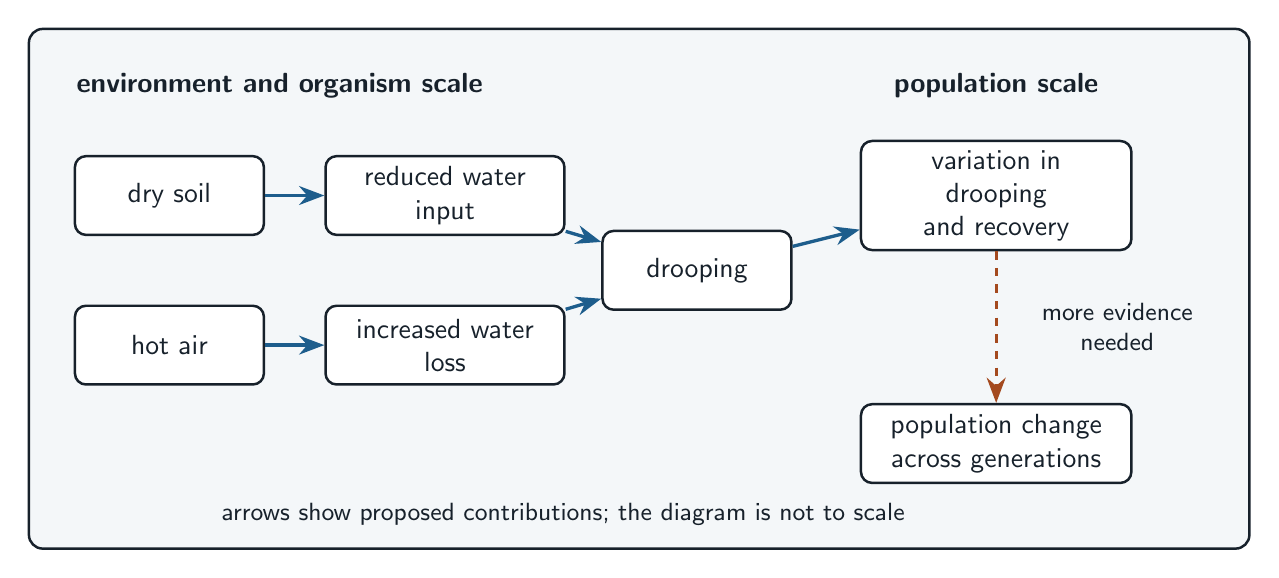
\begin{tikzpicture}[fc text, x=1cm, y=1cm]
  \node[fc panel, minimum width=155mm, minimum height=66mm, anchor=south west] at (0,0) {};
  \node[fc label] at (3.2,5.9) {environment and organism scale};
  \node[fc node] (soil) at (1.8,4.5) {dry soil};
  \node[fc node] (air) at (1.8,2.6) {hot air};
  \node[fc node, text width=28mm] (input) at (5.3,4.5) {reduced water\\input};
  \node[fc node, text width=28mm] (loss) at (5.3,2.6) {increased water\\loss};
  \node[fc node] (droop) at (8.5,3.55) {drooping};
  \draw[fc arrow] (soil)--(input);
  \draw[fc arrow] (air)--(loss);
  \draw[fc arrow] (input)--(droop);
  \draw[fc arrow] (loss)--(droop);
  \node[fc label] at (12.3,5.9) {population scale};
  \node[fc node, text width=32mm] (var) at (12.3,4.5) {variation in\\drooping and recovery};
  \node[fc node, text width=32mm] (pop) at (12.3,1.35) {population change\\across generations};
  \draw[fc arrow] (droop)--(var);
  \draw[fc arrow, draw=fcorange, dashed] (var)--node[fc note, right, text width=28mm] {more evidence\\needed} (pop);
  \node[fc note] at (6.8,.45) {arrows show proposed contributions; the diagram is not to scale};
\end{tikzpicture}
\end{document}
